\documentclass[10pt]{beamer}
%\documentclass[trans]{beamer} %[trans]表示渐进效果pdf压缩打印
\usetheme[sectionpage=progressbar,subsectionpage=progressbar,numbering=counter,progressbar=head]{metropolis}
%numbering=定义页码显示方式;progressbar=定义进度条显示位置
\usepackage{appendixnumberbeamer}
%\usepackage{ctex}%中文字体支持宏包

\usepackage{booktabs}
\usepackage[scale=2]{ccicons}
\usepackage{array}    %支持表格固定宽度
\usepackage{xeCJK}  %中文字体支持宏包
\setCJKmainfont{fzlth.ttf} %方正兰亭黑
%\setsansfont{Ubuntu}
%\setmonofont{Ubuntu Mono}

\usepackage{pgfplots}
\usepgfplotslibrary{dateplot}

\usepackage{xspace}
\newcommand{\themename}{\textbf{\textsc{metropolis}}\xspace}

\title{绪论-光电检测技术}%Photoelectric Detection Technology
\subtitle{Introduction for Photoelectric Detection Technology}
\date{\today}
\author{郎贤礼}
\institute{仪器学院  HFUT}
\titlegraphic{\hfill
\includegraphics[height=2cm]{source/hfutlogo.png}}

\begin{document}

\maketitle

\begin{frame}{Table of contents}
  \setbeamertemplate{section in toc}[sections numbered]
  \tableofcontents[hideallsubsections]
\end{frame}

\section{光电检测的基本概念}
\subsection{光电检测的定义}


%%%%%%%%%%%%%%%%%%%%%%新一页演示文稿%%%%%%%%%%%%%%%%%%%%%%%%%%%%%%%%%%%%

\begin{frame}[fragile]{光电检测的定义}

  \begin{center}
  \large{光电检测是智能信息时代的关键技术}
   \end{center}
   
   现在人类社会已进入人工智能时代AI(Artificial Intelligence)。光电检测是智能信息时代的关键和基础技术。
  
  光信号--->接收、处理、变换---> 电信号\\
  \begin{figure}[htbp]
      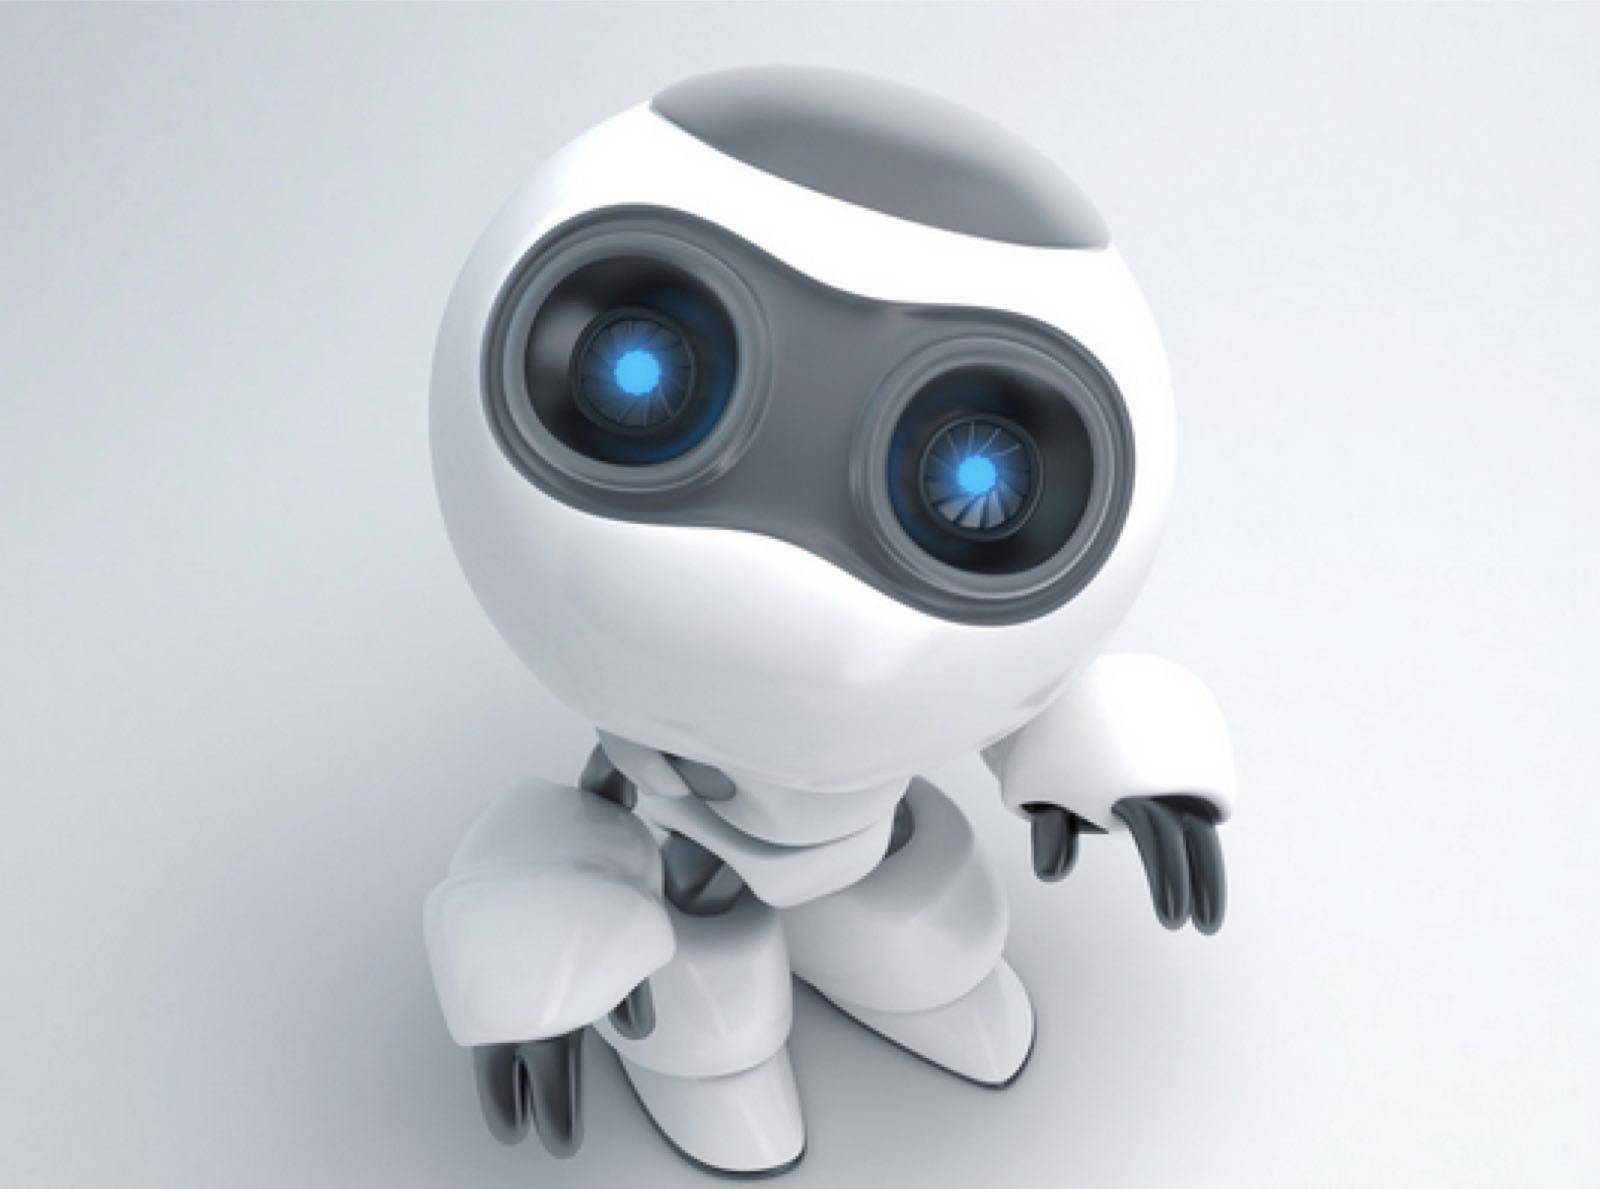
\includegraphics[width=2.0in]{source/ai.jpeg}
  \end{figure}

  
\end{frame}

%%%%%%%%%%%%%%%%%%%%%%新一页演示文稿%%%%%%%%%%%%%%%%%%%%%%%%%%%%%%%%%%%%

\begin{frame}[fragile]{光电检测定义}
\begin{alertblock}{光电检测技术:}
		是利用光电传感器实现各类检测,它将被测量的量转换成光通量,再转换成电量,并综合利用信息传送和处理技术,完成在线和自动测量。

	\end{alertblock}
	
	
	 信息技术:   
  \begin{itemize}
    \item 微电子信息技术(电集成)、光子信息技术(光集成)、光电 信息技术(光电集成)。
    \item 感测技术、通信技术、人工智能与计算机技术、控制技术。
    \item 信息的产生和获取、转换、传输、控制、存储、处理、显示。
 
 \end{itemize}

\end{frame}

%%%%%%%%%%%%%%%%%%%%%%新一页演示文稿%%%%%%%%%%%%%%%%%%%%%%%%%%%%%%%%%%%%

\begin{frame}{光电检测的定义}

课程的重点是光电检测的元器件、系统、方法和应用:

  \begin{itemize}
      \item 重点涉及光电检测的原理和典型应用,所涉及的科学问题、技术特点与难点、各种不同的解决策略与方案和这些方案的优缺点和可能的发展方向.
      \item 要求重点掌握好\alert{基本概念}、各种光电器件的\alert{工作原理与特性}、发展趋势和典型应用;掌握好\alert{光电检测系统的建立方法}
      \item 课程实践性强,在将来的工作、研究中应用广,鼓励积极参与课程实践环节。

  \end{itemize}
  

\end{frame}

%%%%%%%%%%%%%%%%%%%%%%新一页演示文稿%%%%%%%%%%%%%%%%%%%%%%%%%%%%%%%%%%%%
\begin{frame}{光电检测的定义}

    \emph{光电信息技术}:
    \begin{enumerate}[(1)]
        \item<2-| alert@2> 光电源器件(包括激光器)和可控光功能器件及集成
        \item<2-| alert@3> 光通信和综合信息网络
        \item<2-| alert@4> 光频微电子
        \item<2-| alert@5> 光电方法用于瞬态光学观测
        \item<2-| alert@6> \alert{光电传感、光纤传感和图象传感}
        \item<2-| alert@7> \alert{激光、红外、微光探测,定向和制导}
        \item<2-| alert@8> \alert{光电精密测试,在线检测和控制技术}
        \item<2-| alert@9> 混合光电信息处理、识别和图象分析
        \item<2-| alert@10> 光电人工智能和机器视觉
        \item<2-| alert@11> 光(电)逻辑运算和光(电)计算机及光电数据存储
        \item<2-| alert@12> 生物光子学
    \end{enumerate}
\end{frame}
%%%%%%%%%%%%%%%%%%%%%%新一页演示文稿%%%%%%%%%%%%%%%%%%%%%%%%%%%%%%%%%%%%

\begin{frame}{光电检测的定义}
	
	\begin{alertblock}{课程注重:}
	本课程着重在第5、6、7三个方面的一些基本知识,即:\underline{光电检测的元器件、系统、方法和应用}。
	\end{alertblock}
	\begin{itemize}
    
        \item \alert{光电传感、光纤传感和图象传感}
        \item \alert{激光、红外、微光探测,定向和制导}
        \item \alert{光电精密测试,在线检测和控制技术}
        
    \end{itemize}
	
\end{frame}
%%%%%%%%%%%%%%%%%%%%%%新一页演示文稿%%%%%%%%%%%%%%%%%%%%%%%%%%%%%%%%%%%%
\begin{frame}{光电检测技术}
    \begin{itemize}
        \item 检测与测量
        \item 光电传感器:\\
                \begin{itemize}
            \item<2-| alert@2>[+] 基于光电效应,将光信号转换为电信号的一种光电器件
            \item<2-| alert@3>[+] 将非电量转换为与之有确定对应关系的电量输出。
                \end{itemize}
        \item 光电检测技术\\
        是利用光电传感器实现各类检测。它将被测量的量转换成光通量,再转换成电量,并综合利用信息传送和处理技术,完成在线和自动测量.
                
        \item 光电检测系统\\
                \begin{itemize}
            \item<2-| alert@4>[+] 光学变换
            \item<2-| alert@5>[+] 光电变换
            \item<2-| alert@6>[+] 电路处理
                \end{itemize}

    \end{itemize}

\end{frame}
%%%%%%%%%%%%%%%%%%%%%%新一页演示文稿%%%%%%%%%%%%%%%%%%%%%%%%%%%%%%%%%%%%
\begin{frame}{检测的定义}
检测的定义:确定被测对象的属性和量值为目的的全部操作
     \begin{description}
\item[\alert{被测对象}] 宇宙万物(固液气体、动物、植物、天体 ……).
\item[\alert{被测信息}] \begin{itemize}
      \item 物理量(光、电、力、热、磁、声、…).
      \item 化学量(PH、成份…)
      \item 生物量(酶、葡萄糖、…)
      \item ...
                \end{itemize}
\item[\alert{全部操作}] \begin{description}
            \item[检测器具] 传感器、检测仪器、检测装置、检测系统
            \item[检测过程] 信号采集、信号处理、信号显示、信号输出
                        \end{description}
\end{description}

\end{frame}
%%%%%%%%%%%%%%%%%%%%%%新一页演示文稿%%%%%%%%%%%%%%%%%%%%%%%%%%%%%%%%%%%%
\begin{frame}{一个检测的例子}
例:空调机测量控制室温
 
% \frame{\frametitle{Zooming Figures -- Example}
\framezoom<1><2>[border](0cm,0.8cm)(1.5cm,2cm)
\pgfimage[height=2cm]{ac.jpeg}
%\includegraphics[height=6cm]{tiger} is working, too!%
%\centering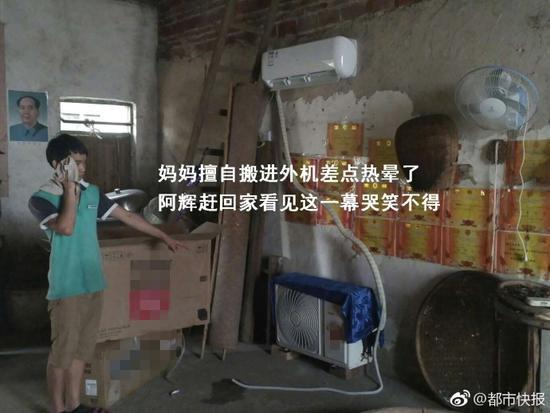
\includegraphics[width=3cm]{ac.jpeg}
%\caption{空调}\label{fig:1}
%\end{figure}
 \begin{description} 
    \item[被测对象] 室内空气
    \item[被测信息] 温度
    \item[被测器具] 温度传感器 热敏电阻 热电偶
    \item[操作过程] 空气 -->热敏电阻 -->电信号  -->显示

 \end{description}
 
 \end{frame}
%%%%%%%%%%%%%%%%%%%%%%新一页演示文稿%%%%%%%%%%%%%%%%%%%%%%%%%%%%%%%%%%%%
\begin{frame}{测量分类}
    

    \begin{alertblock}{直接测量:}
    对仪表读数不经任何运算,直接得出被测量的数值。例如:
    \end{alertblock}
        \begin{itemize}
            \item 长度:直尺、游标卡尺、千分尺
            \item 电压:万用表
            \item 质量:天平
        \end{itemize}
     \begin{alertblock}{间接测量:}
    测量几个与被测量相关的物理量,通过函数关系式计算出被测量。例如:
    \end{alertblock}
        \begin{itemize}
            \item 电功率:$P = I * V$(电流/电压)
            \item 重力加速度:单摆测量(L:摆的线长,T:摆动的周期)
            \begin{equation}
                g=\frac{4\pi^2L}{T^2}
            \end{equation}
            
        \end{itemize}
 \end{frame}    


%%%%%%%%%%%%%%%%%%%%%%新一页演示文稿%%%%%%%%%%%%%%%%%%%%%%%%%%%%%%%%%%%%
\subsection{光电探测器的种类}

\begin{frame}[fragile]{光电探测器的种类}
 \begin{table}[]

 \caption{光电探测器的种类}
\label{table:1}
  \begin{center}
\begin{tabular}{ | m{1.8cm}| m{6.2cm} | } 
\hline
类型& 实例 \\ 
\hline
PN结型 & PN光电二极管(Si,Ge, GaAs)
\newline PIN光电二极管(Si)
\newline 雪崩光电二极管(Si, Ge)
\newline 光电晶体管(Si)
\newline 集成光电传感器和光电晶闸管(Si)
 \\ 
\hline
非PN结型 & 光电元件(CdS, CdSe, Se, PbS)
\newline 热电元件(PZT, LiTaO3, PbTiO3)
 \\ 
\hline
电子管类 & 光电管,摄像管,光电倍增管 \\
\hline
其它类 & 色敏传感器
\newline 固体图象传感器(SI,CCD/MOS/CPD型)
\newline 位置检测用元件(PSD)
\newline 光电池 \\
\hline
\end{tabular}
\end{center}
     
 \end{table}
\end{frame}

\section{光电检测系统组成和方法}
\subsection{光电检测系统组成}
%%%%%%%%%%%%%%%%%%%%%%新一页演示文稿%%%%%%%%%%%%%%%%%%%%%%%%%%%%%%%%%%%%
\begin{frame}{光电检测系统}
    \begin{itemize}
        \item 光电检测技术以激光、红外、光纤等现代光电器件为基础,通过对载有被检测物体信号的光辐射(发射、反射、散射、衍射、折射、透射等)进行检测,即通过光电检测器件接收光辐射并转换为电信号。
        \item 由输入电路、放大滤波等检测电路提取有用的信息,再经过A/D变换接口输入微型计算机运算、处理,最后显示或打印输出所需检测物体的几何量或物理量。

    \end{itemize}


\end{frame}

%%%%%%%%%%%%%%%%%%%%%%新一页演示文稿%%%%%%%%%%%%%%%%%%%%%%%%%%%%%%%%%%%%
\begin{frame}{光电检测系统}
    \begin{figure}[htbp] 
    \centering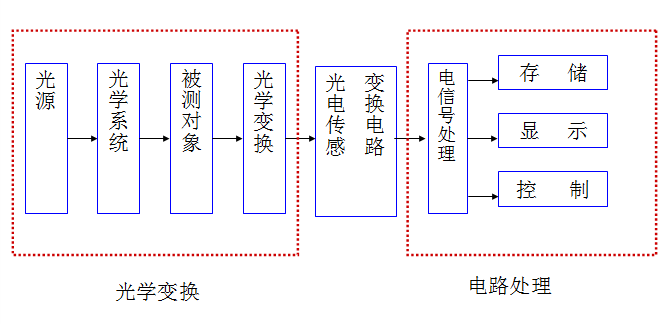
\includegraphics[width=3.5in]{source/intro_oe1.png} 
    \caption{光电检测系统组成}\label{fig:1} 
    \end{figure} 

\end{frame}

%%%%%%%%%%%%%%%%%%%%%%新一页演示文稿%%%%%%%%%%%%%%%%%%%%%%%%%%%%%%%%%%%%
\begin{frame}{光电检测系统}
    \begin{itemize}
        \item 光学变换:\\
            \begin{itemize}
            \item<2-| alert@2>[+] 时域变换:调制振幅、频率、相位、脉宽
            \item<2-| alert@3>[+] 空域变换:光学扫描
            \item<2-| alert@4>[+] 光学参量调制:光强、波长、相位、偏振
            \item<2-| alert@5>[+] 形成能被光电探测器接收,便于后续电学处理的光学信息。
                \end{itemize}
        \item 光电变换:\\
                \begin{itemize}
            \item[+] 光电/热电器件(传感器)、变换电路、前置放大

            \item[+] 将信息变为能够驱动电路处理系统的电信息(电信号的放大和处理)。
                \end{itemize}
        \item 电路处理\\
        \begin{itemize}
            \item[+] 放大、滤波、调制、解调、A/D、D/A、微机与接口、控制。
           \end{itemize}     

    \end{itemize}

\end{frame}
%%%%%%%%%%%%%%%%%%%%%%新一页演示文稿%%%%%%%%%%%%%%%%%%%%%%%%%%%%%%%%%%%%
\begin{frame}{光电检测系统与人操作功能比较}
光电传感部分相当于人身的感觉器官
    \begin{itemize}
        \item 被测物体  ---> 感觉器官  ---> 人脑 ---> 手控  
        \item 被测物体 ---> 光电传感 ---> 微机---> 执行机构
    \end{itemize}
\end{frame}

%%%%%%%%%%%%%%%%%%%%%%新一页演示文稿%%%%%%%%%%%%%%%%%%%%%%%%%%%%%%%%%%%%
\begin{frame}{光电检测系统}
光电检测系统的功能分类
    \begin{itemize}
        \item \alert{测量检查型:}
        \begin{itemize}
            \item<2-| alert@2>[-] 几何量:长度、角度、形状、位置、形变、面积、体积、距离。
            \item<2-| alert@3>[-] 运动量:速度、加速度、振动
            \item<2-| alert@4>[-] 表面形状:光洁度、庇病、伤痕
            \item<2-| alert@5>[-] 工作过程:湿度、流量、压力、物位、PH值、浓度等
            \item<2-| alert@6>[-]  机械量:重量、压力、应变、压强
            \item<2-| alert@7>[-] 电学量:电流、电压、电场、磁场
            \item<2-| alert@8>[-] 光学量:吸收、反射、透射、光度、色度、波长、光谱

        \end{itemize}
        \item \alert{控制跟踪型:}
        \begin{itemize}
            \item<2-| alert@9>[-] 跟踪控制:激光制导,红外制导
            \item<2-| alert@10>[-] 数值控制:自动定位,图形加工形成,数值控制
        \end{itemize}
        \item \alert{图象分析型:}
        \begin{itemize}
            \item[-] 图形检测
            \item[-]图形分析
        \end{itemize}


    \end{itemize}
\end{frame}
%%%%%%%%%%%%%%%%%%%%%%新一页演示文稿%%%%%%%%%%%%%%%%%%%%%%%%%%%%%%%%%%%%


\subsection{光电检测的方法和特点}
%%%%%%%%%%%%%%%%%%%%%%新一页演示文稿%%%%%%%%%%%%%%%%%%%%%%%%%%%%%%%%%%%%
\begin{frame}{光电检测系统与人操作功能比较}
\alert{常见的光电检测方法:}
    \begin{itemize}
        \item 直接作用法
        \item 差动测量法
        \item 补偿测量法
        \item 脉冲测量法
 
    \end{itemize}
    \alert{光电检测技术的特点:}
    \begin{itemize}
        \item<2-| alert@2> 高精度:从地球到月球激光测距的精度达到1米。
        \item<2-| alert@3> 高速度:光速是最快的。
        \item <2-| alert@4>远距离、大量程:遥控、遥测和遥感。
        \item <2-| alert@5>非接触式检测:不改变被测物体性质的条件下进行测量。
        \item<2-| alert@6> 寿命长:光电检测中通常无机械运动部分,故测量装置寿命长,工作可靠、准确度高,对被测物无形状和大小要求。
        \item<2-| alert@7> 数字化和智能化:强的信息处理、运算和控制能力。
 
    \end{itemize}
\end{frame}
%%%%%%%%%%%%%%%%%%%%%%新一页演示文稿%%%%%%%%%%%%%%%%%%%%%%%%%%%%%%%%%%%%


\section{光电检测的应用和发展}
\subsection{光电检测的应用}
%%%%%%%%%%%%%%%%%%%%%%新一页演示文稿%%%%%%%%%%%%%%%%%%%%%%%%%%%%%%%%%%%%
\begin{frame}{光电检测技术的应用}
光电检测技术在工业自
动控制、通讯、信息处理、医疗、生物工程、能源、军事等方面都有广泛的应用
    \begin{enumerate}
        \item 在工业生产领域的应用\\
     \end{enumerate}
        在线检测:零件尺寸、产品缺陷、装配定位….
现代工程装备中,检测环节的成本约占50\~ 70\%
    \begin{columns}
        \begin{column}{0.5\textwidth}
             \begin{figure}[htbp] 
            \centering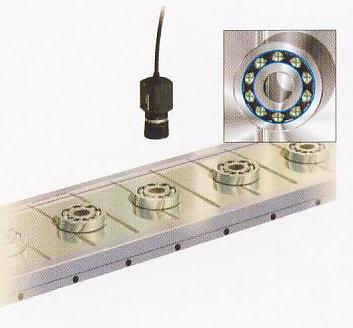
\includegraphics[width=1.75in]{source/intro1.jpg} 
             \caption{检测轴承滚珠脱漏}\label{fig:2} 
             \end{figure}
        \end{column}
        \begin{column}{0.5\textwidth}
        \begin{figure}[htbp] 
            \centering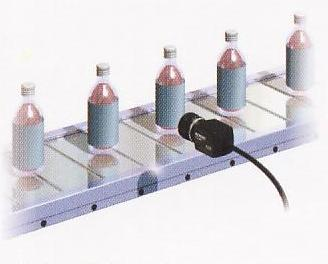
\includegraphics[width=1.75in]{source/intro2.jpg} 
             \caption{检测饮料液位}\label{fig:3} 
            \end{figure}
        \end{column}
        \end{columns}
     
       
    
\end{frame}


%%%%%%%%%%%%%%%%%%%%%%新一页演示文稿%%%%%%%%%%%%%%%%%%%%%%%%%%%%%%%%%%%%
\begin{frame}{检测技术在汽车工业中的应用}
检测技术在汽车工业中的应用。\\
\alert{汽车传感器:}汽车电子控制系统的信息源,关键部件,核心技术内容.普通轿车:约安装几十到近百只传感器;豪华轿车:传感器数量可多达二百余只。 
    \begin{itemize}
        \item 发动机:\\向发动机的电子控制单元(ECU)提供发动机的工作状况信息, 对发动机工作状况进行精确控制.温度、压力、位置、转速、流量、气体浓度和爆震传感器等\\
        \item 底    盘:控制变速器系统、悬架系统、动力转向系统、制动防抱死系统等  车速、踏板、加速度、节气门、发动机转速、水温、油温 
        \item 车    身:提高汽车的安全性、可靠性和舒适性等 
         温度、湿度、风量、日照、加速度、车速、测距、图象等 
    \end{itemize}
\end{frame}
%%%%%%%%%%%%%%%%%%%%%%新一页演示文稿%%%%%%%%%%%%%%%%%%%%%%%%%%%%%%%%%%%%
\begin{frame}{检测技术在汽车工业中的应用}
检测技术在汽车工业中的应用。\\
            \begin{figure}[htbp] 
            \centering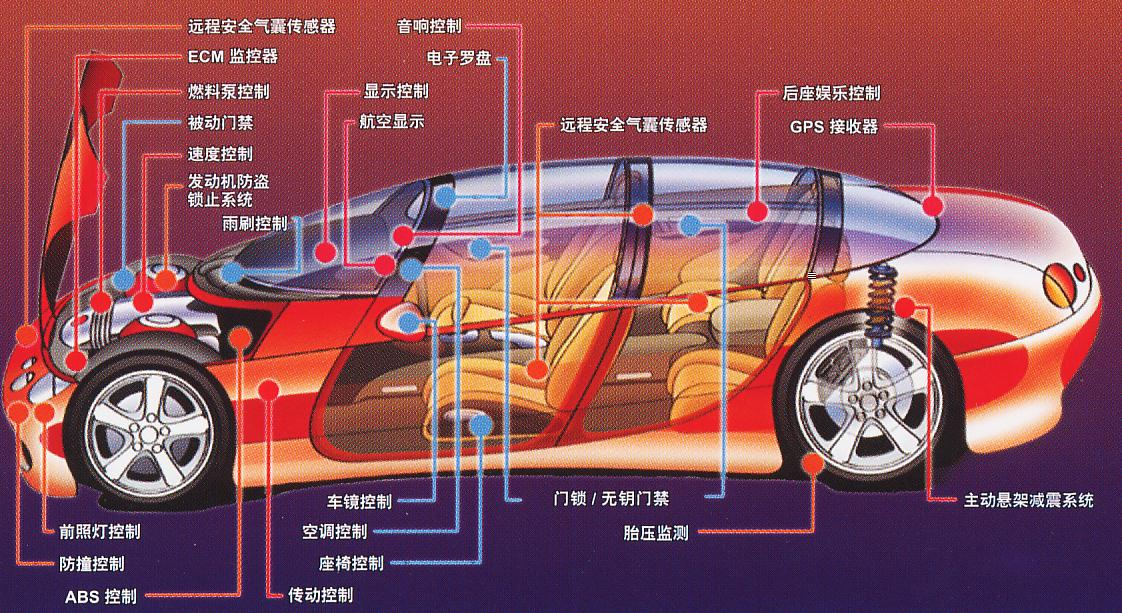
\includegraphics[width=4in]{source/intro3.jpg} \caption{小汽车检测控制系统示意图}\label{fig:3a} 
            \end{figure}
\end{frame}
%%%%%%%%%%%%%%%%%%%%%%新一页演示文稿%%%%%%%%%%%%%%%%%%%%%%%%%%%%%%%%%%%%
\begin{frame}{检测技术在汽车工业中的应用}

    \begin{columns}
        \begin{column}{0.5\textwidth}
        
        \begin{exampleblock}{谷歌自动驾驶汽车:}
        2014年12月中下旬,谷歌首示自动驾驶原型车成品且可全功能运行

      \end{exampleblock}
             \begin{figure}[htbp] 
            \centering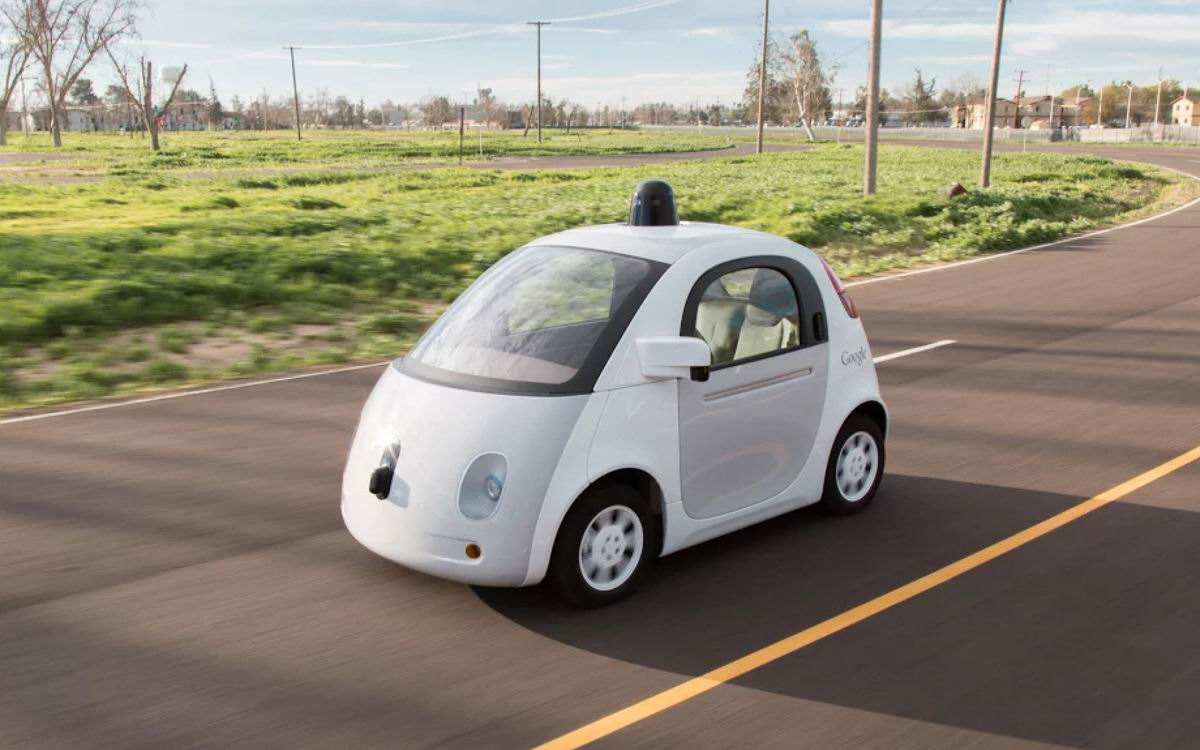
\includegraphics[width=2.25in]{source/intro9.jpg} \caption{谷歌智能驾驶小车}\label{fig:9} 
            \end{figure}
        \end{column}
        \begin{column}{0.5\textwidth}
        \begin{exampleblock}{特斯拉电动汽车:}
       特斯拉设计和制造豪华智能电动车。

      \end{exampleblock}
        \begin{figure}[htbp] 
            \centering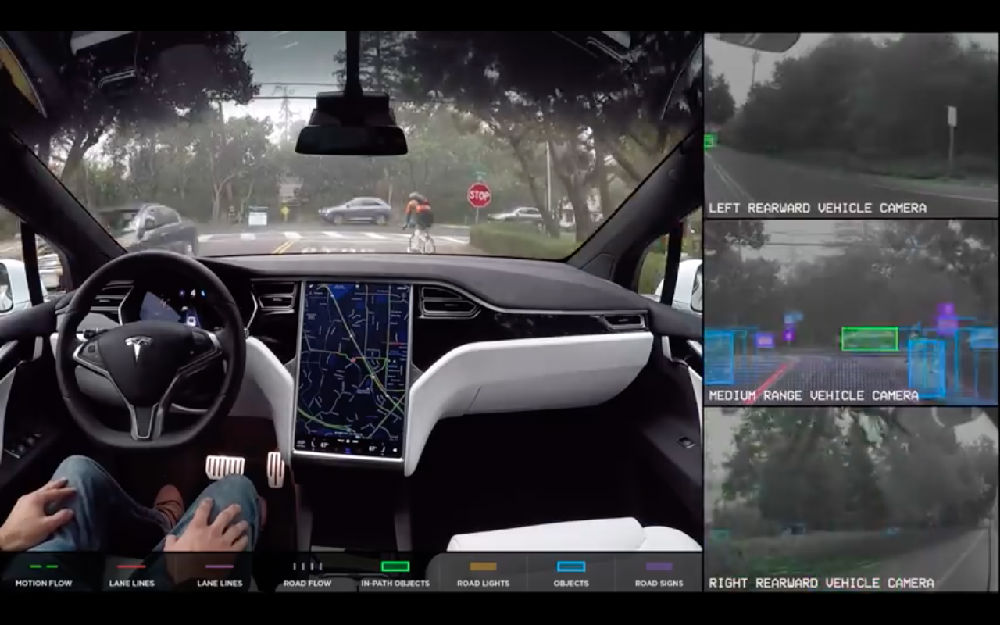
\includegraphics[width=2.25in]{source/intro10.png} \caption{全球首款商用自动驾驶汽车Tesla}\label{fig:10} 
            \end{figure}
        
        \end{column}
        \end{columns}
\end{frame}


%%%%%%%%%%%%%%%%%%%%%%新一页演示文稿%%%%%%%%%%%%%%%%%%%%%%%%%%%%%%%%%%%%
\begin{frame}{检测技术在日常生活中的应用}
2 检测技术在日常生活中的应用
    \begin{itemize}
        \item \alert{家用电器:}
        \begin{itemize}
            \item[-] 数码相机、数码摄像机:自动对焦---红外测距传感器
            \item[-] 自动感应灯:亮度检测---光敏电阻
            \item[-] 空调、冰箱、电饭煲:温度检测---热敏电阻、热电偶
            \item[-] 电话、麦克风:话音转换---驻极电容传感器
            \item[-]  遥控接收:红外检测---光敏二极管、光敏三极管
            \item[-] 可视对讲、可视电话:图像获取---面阵CCD
            

        \end{itemize}
        \item \alert{商务办公:}
        \begin{itemize}
            \item[-] 扫描仪:文档扫描---线阵CCD
            \item[-] 红外传输数据:红外检测---光敏二极管、光敏三极管
        \end{itemize}
        \item \alert{医疗卫生:}
        \begin{itemize}
            \item[-] 数字体温计:接触式---热敏电阻,非接触式---红外传感器
            \item[-]电子血压计:血压检测 --- 压力传感器
            \item[-] 血糖测试仪、胆固醇检测仪 --- 离子传感器
        \end{itemize}


    \end{itemize}
\end{frame}

%%%%%%%%%%%%%%%%%%%%%%新一页演示文稿%%%%%%%%%%%%%%%%%%%%%%%%%%%%%%%%%%%%
\begin{frame}{
检测技术在军事国防领域的应用}
3 检测技术在军事国防领域的应用\\
    \begin{columns}
        \begin{column}{0.6\textwidth}
             \begin{figure}[htbp] 
            \centering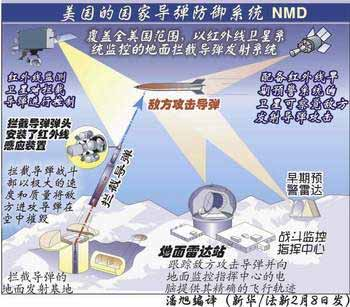
\includegraphics[width=2.5in]{source/intro4.jpg} \caption{美国国家导弹防御计划NMD示意图}\label{fig:4} 
            \end{figure}
        \end{column}
        \begin{column}{0.4\textwidth}
        \begin{itemize}
        \item \alert{美国国家导弹防御计划---NMD}
        \begin{enumerate}[(1)]
            \item 地基拦截器
            \item 早期预警系统
            \item 前沿部署(如雷达)
            \item 管理与控制系统
            \item 卫星红外线监测系统
     

        \end{enumerate}
        \item \alert{监测系统:}
         探测和发现敌人导弹的发射并追踪导弹的飞行轨道;
        \item \alert{拦截器:}
        能识别真假弹头,敌友方
        \end{itemize}
        \end{column}
        \end{columns}
\end{frame}

%%%%%%%%%%%%%%%%%%%%%%新一页演示文稿%%%%%%%%%%%%%%%%%%%%%%%%%%%%%%%%%%%%
\begin{frame}{
3 检测技术在军事国防领域的应用}
现在每个国家都很重视单兵装备的的问题,发展先进的个人装备对人的生命安全和战略战术有着重要的意义。
    \begin{columns}
        \begin{column}{0.6\textwidth}
        
        \begin{itemize}
        \item 夜视瞄准机系统:非冷却红外传感器技术

        \item 激光测距仪:可精确的定位目标。
        \end{itemize}
             \begin{figure}[htbp] 
            \centering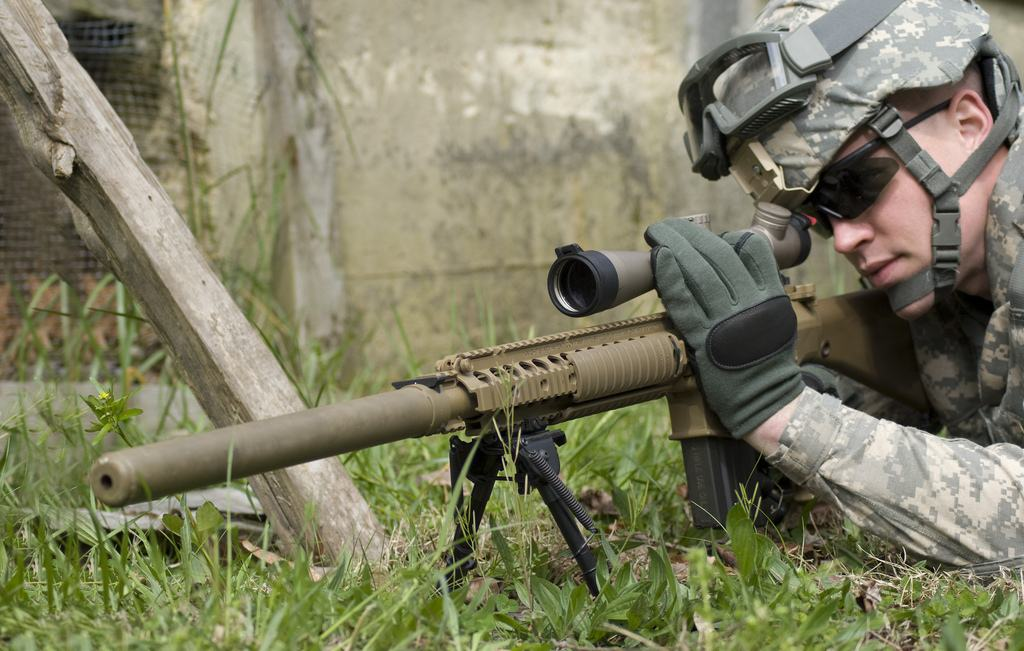
\includegraphics[width=2.5in]{source/intro5.jpg} \caption{美国单兵作战武器a}\label{fig:5} 
            \end{figure}
        \end{column}
        \begin{column}{0.4\textwidth}
        \begin{figure}[htbp] 
            \centering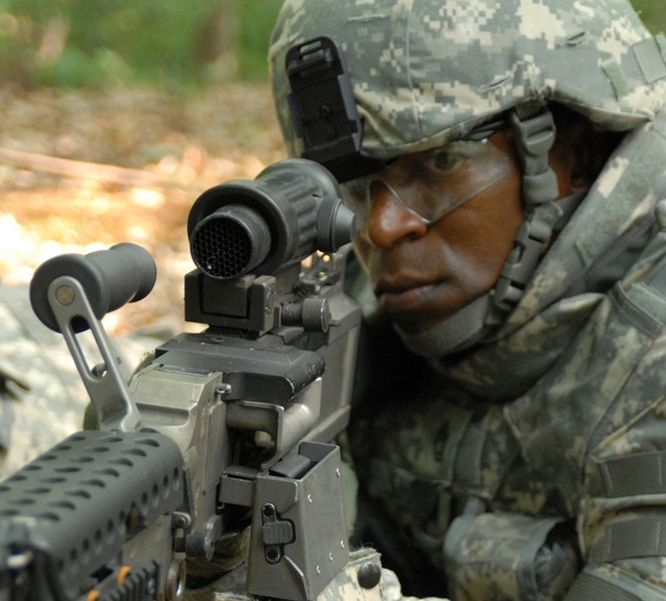
\includegraphics[width=2.0in]{source/intro6.jpg} \caption{美国单兵作战武器b}\label{fig:6} 
            \end{figure}
        
        \end{column}
        \end{columns}
\end{frame}
%%%%%%%%%%%%%%%%%%%%%%新一页演示文稿%%%%%%%%%%%%%%%%%%%%%%%%%%%%%%%%%%%%
\begin{frame}{4检测技术在航天领域的应用}

    \begin{columns}
        \begin{column}{0.5\textwidth}
        
        \begin{exampleblock}{阿波罗10:}
        火箭部分---2077个传感器\\
        飞船部分---1218个传感器

      \end{exampleblock}
             \begin{figure}[htbp] 
            \centering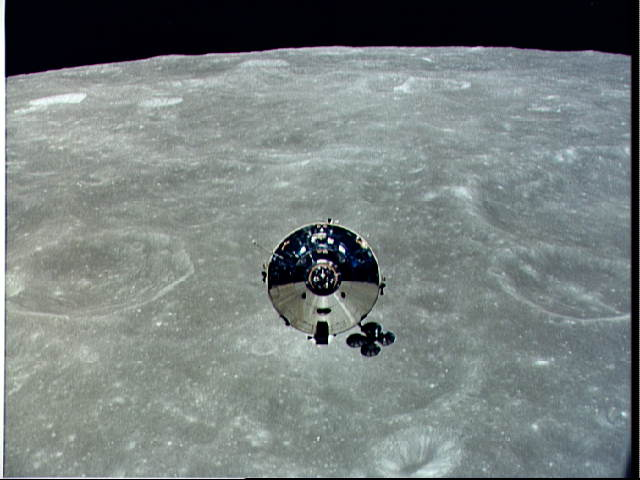
\includegraphics[width=2.25in]{source/intro7.jpg} \caption{阿波罗10飞船}\label{fig:7} 
            \end{figure}
        \end{column}
        \begin{column}{0.5\textwidth}
        \begin{exampleblock}{神州飞船:}
        185台(套)仪器装置\\
        检测参数---加速度、温度、压力、 振动、流量、应变、  声学

      \end{exampleblock}
        \begin{figure}[htbp] 
            \centering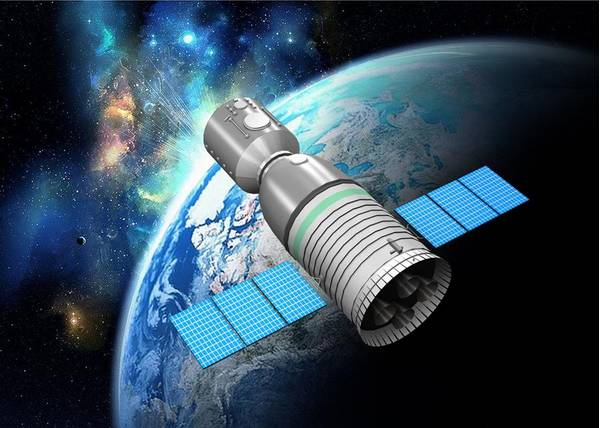
\includegraphics[width=2.25in]{source/intro8.jpg} \caption{神州飞船}\label{fig:8} 
            \end{figure}
        
        \end{column}
        \end{columns}
\end{frame}

%%%%%%%%%%%%%%%%%%%%%%新一页演示文稿%%%%%%%%%%%%%%%%%%%%%%%%%%%%%%%%%%%%





\subsection{光电检测的发展趋势}
%%%%%%%%%%%%%%%%%%%%%%新一页演示文稿%%%%%%%%%%%%%%%%%%%%%%%%%%%%%%%%%%%%
\begin{frame}{光电检测技术发展趋势}
光电检测技术发展趋势
    \begin{enumerate}[(1)]
    \item<2-| alert@2>纳米、亚纳米高精度的光电测量新技术。
    \item<2-| alert@3>小型、快速的微型光、机、电检测系统。
    \item<2-| alert@4>非接触、快速在线测量。
    \item<2-| alert@5> 微空间三维测量技术和大空间三维测量技术。
    \item<2-| alert@6> 闭环控制的光电检测系统,实现光电测量与光电控制一体化。
    \item<2-| alert@7> 向人们无法触及的领域发展。
    \item<2-| alert@8> 光电跟踪与光电扫描测量技术。
    \item<2-| alert@9> 智能检测和智能感知
    \end{enumerate}
\end{frame}
%%%%%%%%%%%%%%%%%%%%%%新一页演示文稿%%%%%%%%%%%%%%%%%%%%%%%%%%%%%%%%%%%%
\section{课程愿景}
%%%%%%%%%%%%%%%%%%%%%%新一页演示文稿%%%%%%%%%%%%%%%%%%%%%%%%%%%%%%%%%%%%
\begin{frame}{Our Philosophy}
课程愿景
      \begin{columns}
        \begin{column}{0.6\textwidth}
        
        \begin{enumerate}[(1)]
    \item<2-| alert@2>认识到“光电检测很有用”
    \item<2-| alert@3>掌握光电检测的原理与方法并学会构建光电检测系统
    \item<2-| alert@4>Have fun!
    
    \end{enumerate}
        \end{column}
        \begin{column}{0.4\textwidth}
        \begin{figure}[htbp] 
        \centering
\includegraphics[width=2.0in]{source/intro11.jpg} 
    %\caption{光电检测系统组成}\label{fig:1} 
        \end{figure} 
        
        \end{column}
        \end{columns}
    
    
    
\end{frame}

%%%%%%%%%%%%%%%%%%%%%%新一页演示文稿%%%%%%%%%%%%%%%%%%%%%%%%%%%%%%%%%%%%

\section{成绩评定}
%%%%%%%%%%%%%%%%%%%%%%新一页演示文稿%%%%%%%%%%%%%%%%%%%%%%%%%%%%%%%%%%%%
\begin{frame}{Grading policy}
成绩评定
    \begin{columns}
        \begin{column}{0.6\textwidth}
        
        \begin{itemize}
    \item Midterm Exam: \alert{
30\%}
    \item Final Exam: \alert{40\%}
    \item Assignments: \alert{10\%}
    \item Experiment Report: \alert{10\%}
    \item Attendance: \alert{10\%}
    \end{itemize}
        \end{column}
        \begin{column}{0.4\textwidth}
        \begin{figure}[htbp] 
        \centering
\includegraphics[width=1.0in]{source/intro12.jpg} 
    %\caption{光电检测系统组成}\label{fig:1} 
        \end{figure} 
        
        \end{column}
        \end{columns}
    
    
\end{frame}

\section{参考书目}


\begin{frame}{References}
   \begin{columns}
        \begin{column}{0.6\textwidth}
        
         \begin{itemize}
        \item \alert{课程所用教材:}\cite{coursebook}
        \begin{itemize}
            \item[-] 《光电检测技术与应用》郭培源
        \end{itemize}
        \item \alert{参考书目:}\cite{cbook1,cbook2,cbook3}
        \begin{itemize}
            \item[-] 《光电检测技术》曾光宇等编著
            \item[-] 《激光光电检测》吕海宝等编著
            \item[-] 《光电检测技术》雷玉堂等编著
        \end{itemize}
    \end{itemize}
        \end{column}
        \begin{column}{0.4\textwidth}
        \begin{figure}[htbp] 
        \centering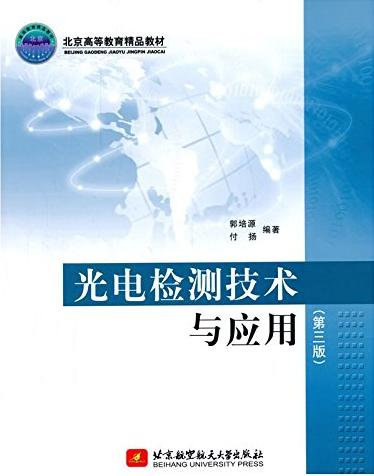
\includegraphics[width=2.0in]{source/pdt.jpg} 
    %\caption{光电检测系统组成}\label{fig:1} 
        \end{figure} 
        
        \end{column}
        \end{columns}
  
 
\end{frame}


\begin{frame}[standout]
  Questions?
\end{frame}

\appendix

\begin{frame}[fragile]{Backup slides}
  Sometimes, it is useful to add slides at the end of your presentation to
  refer to during audience questions.

  The best way to do this is to include the \verb|appendixnumberbeamer|
  package in your preamble and call \verb|\appendix| before your backup slides.

  \themename will automatically turn off slide numbering and progress bars for
  slides in the appendix.
\end{frame}

\begin{frame}[allowframebreaks]{参考书目}

  \bibliography{demo}
  \bibliographystyle{unsrt}%{ieeetr}%{abbrv}

\end{frame}

\end{document}

